\documentclass[aspectratio=169,12pt]{beamer}
\usepackage[T1]{fontenc}
\usepackage{lmodern}
\usepackage{tikz}
\usetikzlibrary{arrows.meta,positioning,calc}
\usepackage{booktabs,tabularx,array,amsmath,graphicx}
\usepackage{pgfplots}
\pgfplotsset{compat=1.18}
\geometry{paperwidth=192mm,paperheight=108mm}
\graphicspath{{assets/}}

\definecolor{Primary}{RGB}{103,58,183}
\definecolor{Deep}{RGB}{69,39,160}
\definecolor{Light}{RGB}{179,157,219}
\definecolor{Pale}{RGB}{243,238,250}
\definecolor{Ink}{RGB}{36,33,54}
\definecolor{Muted}{RGB}{100,94,115}
\setbeamercolor{normal text}{fg=Ink,bg=white}
\setbeamercolor{structure}{fg=Primary}
\setbeamercolor{frametitle}{fg=Deep}
\setbeamercolor{title}{fg=Deep}
\setbeamercolor{itemize item}{fg=Primary}
\setbeamercolor{itemize subitem}{fg=Primary}
\setbeamercolor{block title}{fg=Deep,bg=Pale}
\setbeamercolor{block body}{fg=Ink,bg=Pale}
\setbeamercolor{footline}{fg=Muted}
\setbeamerfont{frametitle}{size=\Large,series=\bfseries}
\setbeamerfont{title}{size=\LARGE,series=\bfseries}
\setbeamersize{text margin left=8mm,text margin right=8mm}
\setbeamertemplate{navigation symbols}{}
\setbeamertemplate{itemize item}{\small\textbullet}
\newcommand{\slidetitle}[1]{%
  \vspace*{2mm}%
  {\usebeamerfont{frametitle}\color{Deep}\strut #1\strut\par}%
  \vskip1mm\hbox{\color{Light}\rule{\textwidth}{0.45pt}}\vskip1mm}
\setbeamertemplate{footline}{%
  \hspace{8mm}\usebeamerfont{footline}\fontsize{6.5}{8}\selectfont
  Arush Ram Anandh\hfill LLM-guided drone path planning\hfill
  \insertframenumber/\inserttotalframenumber\hspace{8mm}\vspace{3mm}}
\setbeamertemplate{note page}[plain]
\ifdefined\shownotes\setbeameroption{show only notes}\else\setbeameroption{hide notes}\fi
\hypersetup{colorlinks=true,urlcolor=Primary,pdfauthor={Arush Ram Anandh},
  pdftitle={LLM-Guided Drone Path Planning: A Critical Discussion}}
\title{LLM-Guided Drone\\Path Planning}
\subtitle{A critical discussion of Farooq et al.}
\author{Arush Ram Anandh}
\date{}

\newcommand{\source}[1]{\par\vfill{\fontsize{6.5}{8}\selectfont\color{Muted}Source: #1\par}}
\newcommand{\labeltext}[1]{{\color{Deep}\bfseries #1}}
\newcommand{\emphasis}[1]{\begin{beamercolorbox}[sep=2mm,wd=\linewidth]{block body}#1\end{beamercolorbox}}
\newcommand{\smallbody}{\fontsize{10}{12.5}\selectfont}
\newcommand{\compactbody}{\fontsize{9}{11}\selectfont}
\newcolumntype{Y}{>{\raggedright\arraybackslash}X}
\tikzset{flow/.style={draw=Light,fill=Pale,rounded corners=1pt,align=center,
  font=\fontsize{9}{11}\selectfont,inner sep=4pt},
  link/.style={-{Latex[length=1.8mm]},draw=Primary,thick}}

\begin{document}

\begin{frame}[plain,noframenumbering]
  \vspace{7mm}
  {\color{Primary}\rule{16mm}{1.2pt}}\par\vspace{5mm}
  {\usebeamerfont{title}\color{Deep}\inserttitle\par}
  \vspace{3mm}
  {\color{Muted}\small A critical discussion of Farooq et al.\par}
  \vspace{7mm}
  {\normalsize\insertauthor\par}
  \vfill
  {\fontsize{9}{12}\selectfont\color{Muted}
  Paper: \emph{Goal-Oriented Intelligence Path Planning for LLMs\\
  Based Drone in Adversarial Conditions}\par}
  \vspace{5mm}
  \note{Introduce the paper as an integration concept with preliminary simulation evidence. The talk distinguishes what the authors report, what we infer, and what they leave unspecified. Eight substantive slides take approximately 18.5 minutes.}
\end{frame}

\begin{frame}[t]
  \slidetitle{Can foundation models help drones navigate?}
  \vspace{2mm}
  \begin{columns}[T,onlytextwidth]
  \begin{column}{0.54\textwidth}
    \begin{itemize}\setlength\itemsep{3mm}
      \item Reach a destination while avoiding obstacles.
      \item Unfamiliar or changing environments motivate adaptive navigation.
      \item The paper explores LLMs/VLMs for waypoint planning using visual context.
    \end{itemize}
  \end{column}
  \begin{column}{0.43\textwidth}
    \centering
    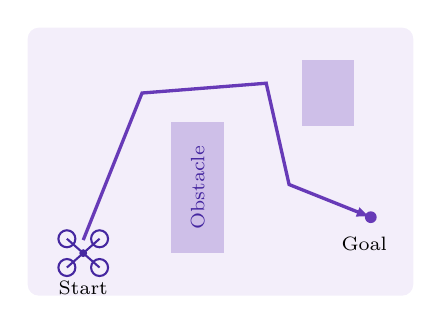
\begin{tikzpicture}[x=0.83cm,y=0.83cm]
      \fill[Pale,rounded corners=4pt] (0,0) rectangle (5.9,4.1);
      \fill[Light!65] (2.2,0.65) rectangle (3.0,2.65);
      \fill[Light!65] (4.2,2.6) rectangle (5.0,3.6);
      \node[rotate=90,font=\scriptsize,text=Deep] at (2.6,1.65) {Obstacle};
      \draw[link,line width=1.2pt] (0.85,0.85)--(1.75,3.1)--(3.65,3.25)--(4.0,1.7)--(5.25,1.2);
      \begin{scope}[shift={(0.85,0.65)},draw=Deep,line width=0.75pt]
        \draw (-0.25,-0.22)--(0.25,0.22) (-0.25,0.22)--(0.25,-0.22);
        \foreach \x in {-0.25,0.25}\foreach \y in {-0.22,0.22}\draw (\x,\y) circle (0.13);
        \fill[Deep] (0,0) circle (0.06);
      \end{scope}
      \node[font=\scriptsize] at (0.85,0.12) {Start};
      \fill[Primary] (5.25,1.2) circle (0.09);
      \node[font=\scriptsize,below] at (5.15,1.05) {Goal};
    \end{tikzpicture}\par
    {\fontsize{7}{9}\selectfont\color{Muted}Illustrative route, not an experimental result\par}
  \end{column}
  \end{columns}
  \vspace{4mm}
  \emphasis{\labeltext{Research question}\par\smallskip
    What useful role can a foundation model play in a drone navigation system?}
  \source{\texttt{paper.pdf}, pp. 1, 3--4.}
  \note{Timing: 1.5 minutes. Conventional geometric planners search for routes under a representation of free space. Foundation models may contribute instruction understanding and contextual decisions. RRT is a classical randomized motion-planning algorithm, not machine learning. This paper does not establish superior navigation. GPS-denied navigation motivates the work, but the displayed evaluation uses simulated obstacle environments. The drawing is a schematic only.}
\end{frame}

\begin{frame}[t]
  \slidetitle{Why LLMs? The authors' broader motivation}
  \vspace{5mm}
  \begin{columns}[T,onlytextwidth]
  \begin{column}{0.31\textwidth}
    
\begin{tikzpicture}[draw=Primary,line width=0.9pt]
      \draw (0,0)--(0.75,0.6)--(1.5,0)--cycle;
      \foreach \p in {(0,0),(0.75,0.6),(1.5,0)}\draw[fill=white] \p circle (0.13);
    \end{tikzpicture}\par\vspace{3mm}
    \labeltext{Coordination}\par\vspace{2mm}
    \smallbody Multi-UAV communication, mission planning and information exchange.
  \end{column}
  \begin{column}{0.32\textwidth}
    
\begin{tikzpicture}[draw=Primary,line width=0.9pt]
      \draw[rounded corners=2pt] (0,0) rectangle (1.4,0.65);
      \draw (0.25,0.43)--(1.15,0.43) (0.25,0.23)--(0.85,0.23);
      \draw (0.3,0)--(0.15,-0.18)--(0.65,0);
    \end{tikzpicture}\par\vspace{3mm}
    \labeltext{Contextual reasoning}\par\vspace{2mm}
    \smallbody Interpret instructions, observations, unexpected events and anomalies.
  \end{column}
  \begin{column}{0.30\textwidth}
    
\begin{tikzpicture}[draw=Primary,line width=0.9pt]
      \draw[link] (0,0)--(0.45,0)--(0.45,0.65)--(1.4,0.65);
      \draw (0.85,-0.1) rectangle (1.15,0.3);
    \end{tikzpicture}\par\vspace{3mm}
    \labeltext{Adaptation}\par\vspace{2mm}
    \smallbody Respond to changing obstacles with goal-directed navigation decisions.
  \end{column}
  \end{columns}
  \vspace{8mm}
  {\smallbody\color{Muted}These capabilities motivate the paper. Its experiments cover a narrower task.\par}
  \vspace{3mm}
  \emphasis{\labeltext{Specific experiment}\par\smallskip
    Vision-guided waypoint generation in simulated obstacle environments.}
  \source{\texttt{paper.pdf}, p. 3, broader motivation; pp. 4--5, experimental scope.}
  \note{Timing: 2 minutes. Multi-UAV communication, information exchange, mission coordination and emergency response appear in the authors' broader discussion. Treat these as motivations, not experimentally demonstrated contributions. The reported experiment concerns visual-context-guided waypoint generation in simulation. LLM means large language model; VLM means vision-language model; UAV means unmanned aerial vehicle.}
\end{frame}

\begin{frame}[t]
  \slidetitle{Proposed architecture: observations to flight}
  \vspace{1mm}
  \begin{columns}[T,onlytextwidth]
  \begin{column}{0.72\textwidth}
    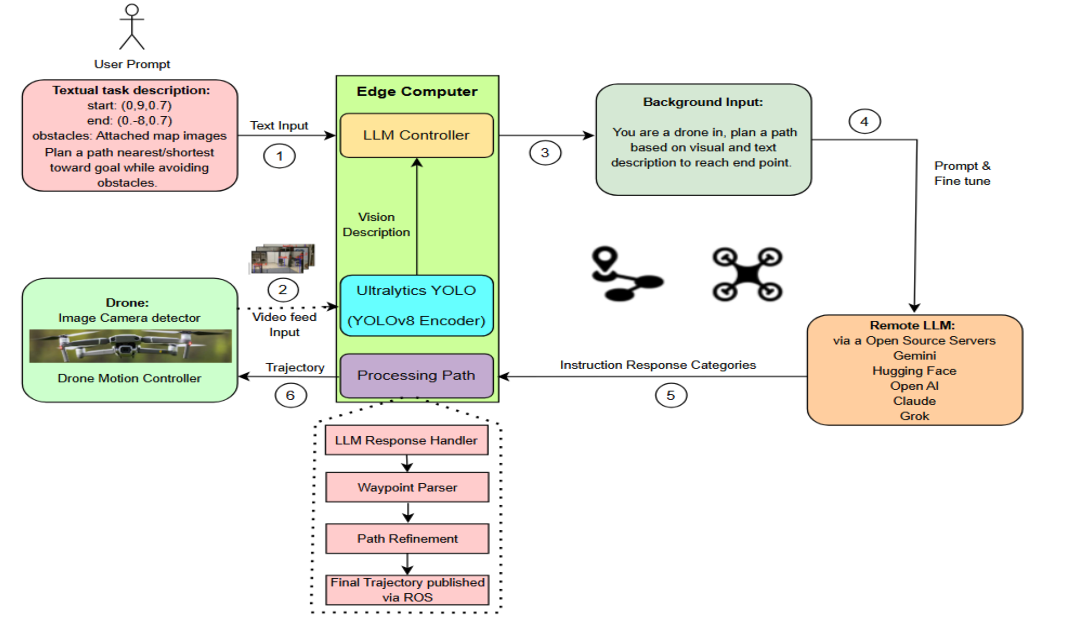
\includegraphics[width=\linewidth,height=70mm,keepaspectratio]{figure3.pdf}\par
    {\fontsize{7}{9}\selectfont\color{Muted}Original Figure 3, cropped from the paper\par}
  \end{column}
  \begin{column}{0.26\textwidth}
    \smallbody
    \labeltext{Reading guide}\par\vspace{1mm}
    \begin{enumerate}\setlength\itemsep{1.3mm}
      \item Start, goal, instructions and camera input
      \item YOLOv8 object detection
      \item Constructed input to remote LLM/VLM
      \item Parse and interpolate waypoints
      \item ROS to motion controller
    \end{enumerate}
    \vspace{5mm}
    \emphasis{\compactbody\labeltext{Not specified:} the exact arrangement of the fine-tuned and remotely prompted models.}
  \end{column}
  \end{columns}
  \source{\texttt{paper.pdf}, p. 4, Fig. 3 and methodology; p. 5, RGB/depth observations.}
  \note{Timing: 3 minutes. Read the original diagram using the five-step guide, which groups its six numbered arrows into functional stages. YOLOv8 is a learned detector, not by itself a 3D coordinate estimator. RGB and depth images are mentioned on p. 5, but the transformation into obstacle world coordinates is unexplained. Updated observations may support replanning, but neither cadence nor trigger is specified. The paper describes interpolation with approximately 0.1 m spacing. This adds points along existing segments and guarantees neither smoothness, obstacle avoidance nor dynamically feasible flight. ROS carries the final trajectory. The motion-controller type is not identified; do not call it PID. The remote-server labels in the source figure do not identify which model generated Table I.}
\end{frame}

\begin{frame}[t]
  \slidetitle{Fine-tuning, prompt structure and inference}
  \vspace{1mm}
  \begin{columns}[T,onlytextwidth]
  \begin{column}{0.48\textwidth}
    \labeltext{Training}\par\vspace{1.5mm}
    \centering
    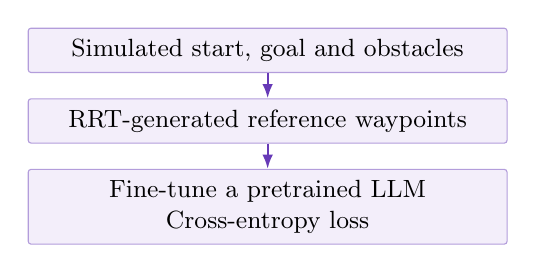
\begin{tikzpicture}[node distance=3.2mm]
      \node[flow,text width=5.8cm] (a) {Simulated start, goal and obstacles};
      \node[flow,text width=5.8cm,below=of a] (b) {RRT-generated reference waypoints};
      \node[flow,text width=5.8cm,below=of b] (c) {Fine-tune a pretrained LLM\\Cross-entropy loss};
      \draw[link] (a)--(b);\draw[link] (b)--(c);
    \end{tikzpicture}
  \end{column}
  \begin{column}{0.48\textwidth}
    \labeltext{Inference}\par\vspace{1.5mm}
    \centering
    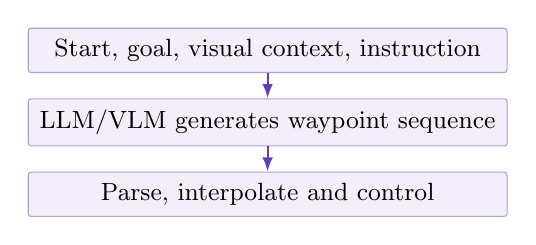
\begin{tikzpicture}[node distance=3.2mm]
      \node[flow,text width=5.8cm] (a) {Start, goal, visual context, instruction};
      \node[flow,text width=5.8cm,below=of a] (b) {LLM/VLM generates waypoint sequence};
      \node[flow,text width=5.8cm,below=of b] (c) {Parse, interpolate and control};
      \draw[link] (a)--(b);\draw[link] (b)--(c);
    \end{tikzpicture}
  \end{column}
  \end{columns}
  \vspace{1mm}
  {\fontsize{10}{12}\selectfont
  \[\underbrace{\mathrm{Input}=\mathrm{Start}+\mathrm{Goal}+\mathrm{Visual\ Map}+\mathrm{Instruction}}_{\text{Paper's input expression, abbreviated from Eq. (1)}}\]}
  \vspace{0mm}
  {\compactbody
  \noindent\labeltext{Reported:} 105 epochs; training loss $\approx 0.15$ near epoch 65; three visual-map examples for few-shot prompting.\par\vspace{2.5mm}
  \labeltext{Not specified:} model identity/method, dataset size/split, coordinate formatting, exact prompt, visual-to-spatial conversion, or which model produced the aggregate results.\par\vspace{1.7mm}
  \labeltext{Inconsistency:} reference-path clearance is 2 m on p. 4 and 1.2 m on p. 5.}
  \source{\texttt{paper.pdf}, pp. 4--5, methodology, Eq. (1) and training description. Flows summarize the prose.}
  \note{Timing: 3.5 minutes. RRT is a classical randomized tree search in free space. Ordinary RRT does not guarantee shortest paths, despite the paper's wording. The paper reports RRT waypoint targets and fine-tuning a pretrained LLM with cross-entropy. This suggests imitation of reference outputs, but exact training inputs, target formatting, tokenization and parameter-update method remain unclear. The paper also describes few-shot prompting of commercial LLMs/VLMs with three visual-map examples. It does not adequately connect the two accounts or attribute aggregate results to a specific system. The two flows organize the reported prose; they are not a verified implementation diagram. The displayed input expression abbreviates the paper's own Eq. (1), not a new optimization objective. Reported training loss alone does not establish generalization. Flag the 2 m versus 1.2 m clearance discrepancy without selecting a preferred value.}
\end{frame}

\begin{frame}[t]
  \slidetitle{Experimental results: what was measured?}
  \vspace{2mm}
  \begin{columns}[T,onlytextwidth]
  \begin{column}{0.60\textwidth}
    \labeltext{Table I: reported simulation results}\par\vspace{3mm}
    \fontsize{9}{11}\selectfont
    \setlength\tabcolsep{3.5pt}\renewcommand\arraystretch{1.45}
    \begin{tabularx}{\linewidth}{@{}Yrrrr@{}}
    \toprule
    Environment & \shortstack{Obstacles} & \shortstack{Moving\\obstacles} & \shortstack{Success\\rate} & \shortstack{Mean\\time (s)}\\
    \midrule
    Simple   & 8--10  & 3  & 95.0\% & 65.7\\
    Moderate & 10--12 & 7  & 92.0\% & 65.4\\
    Complex  & 12--16 & 10 & 91.5\% & 69.2\\
    Dynamic  & 16--20 & 12 & 89.0\% & 72.0\\
    \bottomrule
    \end{tabularx}\par
    \vspace{3mm}
    {\smallbody Success decreases from \labeltext{95\% to 89\%} across the reported categories.\par}
  \end{column}
  \begin{column}{0.37\textwidth}
    \centering
    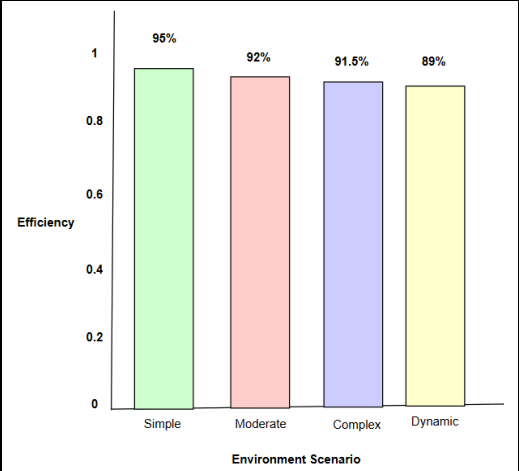
\includegraphics[width=0.95\linewidth,height=36mm,keepaspectratio]{figure4.pdf}\par
    {\fontsize{7}{9}\selectfont\color{Muted}Original Figure 4\par}
  \end{column}
  \end{columns}
  \vspace{4mm}
  \emphasis{\compactbody
    \labeltext{Evidence limits}\par\smallskip
    All four categories list moving obstacles. Formal difficulty definitions and obstacle motion models are unspecified.\par\smallskip
    Trial counts and uncertainty are unreported. Figure 4 calls success rates ``efficiency'' without defining a separate path-efficiency metric.}
  \source{\texttt{paper.pdf}, p. 5, Table I and Fig. 4; p. 6, conclusion claims.}
  \note{Timing: 3 minutes. Table I reports obstacle ranges, moving-obstacle counts, average completion times and success percentages. Every category includes moving obstacles, including Simple. Formal category definitions, obstacle velocities and motion models are not provided. The trial count and success criterion are not operationally specified, and there are no error bars, standard deviations or confidence intervals. Mean completion time is not monotonic from Simple to Moderate. The six-percentage-point success decrease is descriptive, not proof of an inverse proportionality or a statistically established effect. Figure 4 reuses the four success percentages under an efficiency label. No direct RRT comparison or path-optimality metric accompanies these results. The real-world, GPS-denied and bad-weather claims exceed the evaluation shown.}
\end{frame}

\begin{frame}[t]
  \slidetitle{What is missing from the evaluation?}
  \vspace{1mm}
  \smallbody\renewcommand\arraystretch{1.35}
  \begin{tabularx}{\textwidth}{@{}>{\raggedright\arraybackslash}p{35mm}Y@{}}
    \toprule
    \labeltext{Dimension} & \labeltext{Missing or unclear}\\
    \midrule
    Reproducibility & Model identity, dataset size, trial count and splits\\
    Baselines & Controlled comparisons with RRT/RRT*, A* or other planners\\
    Safety & Collision rates, segment validation and measured clearance\\
    Path quality & Length, optimality, smoothness and energy\\
    Real-time operation & Inference latency, replanning frequency and compute\\
    Generalization & Unseen environments, sensor noise and physical flight\\
    \bottomrule
  \end{tabularx}\par
  \vspace{4mm}
  \emphasis{What advantage does the learned planner demonstrate over the planner used to generate its reference paths?}
  \source{\texttt{paper.pdf}, pp. 4--6. Evaluation gaps identified in this discussion.}
  \note{Timing: 2 minutes. Missing evidence is not evidence that the system fails. The architecture is interesting, but the evaluation does not isolate an LLM contribution. A useful controlled experiment would compare planners on identical scenes, starts, goals and constraints, reporting trial counts and uncertainty. Safety needs explicit collision checking and measured clearance, beyond a goal-reaching percentage. Real-time feasibility needs latency and a replanning schedule. Generalization needs held-out scenes and sensor disturbances, followed by appropriately controlled physical validation. These are proposed evaluation requirements, not tests the paper reports.}
\end{frame}

\begin{frame}[t]
  \slidetitle{Alternative planning methods and extensions}
  \vspace{1mm}
  {\fontsize{8}{10}\selectfont\color{Primary}\bfseries Our analysis / proposed extensions\par}
  \vspace{1.5mm}
  \fontsize{9}{11}\selectfont\renewcommand\arraystretch{1.35}
  \begin{tabularx}{\textwidth}{@{}>{\raggedright\arraybackslash}p{39mm}>{\raggedright\arraybackslash}p{51mm}Y@{}}
    \toprule
    \labeltext{Approach} & \labeltext{Role} & \labeltext{Why include it?}\\
    \midrule
    A*, RRT, RRT* & Classical geometric planning & Feasibility, path cost and a reproducible baseline\\
    Model Predictive Control (MPC) & Receding-horizon planning/control & Dynamic obstacles and control constraints\\
    Reinforcement Learning (RL) & Learned navigation policies & Learning from interaction and adaptation\\
    Hybrid LLM + classical planner & Semantic decisions with geometric validation & Test added value while retaining explicit safety checks\\
    \bottomrule
  \end{tabularx}\par
  \vspace{4mm}
  \labeltext{Proposed hybrid pipeline}\par\vspace{2mm}
  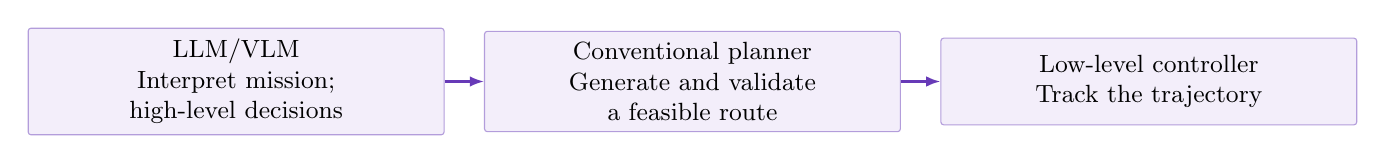
\begin{tikzpicture}
    \node[flow,text width=50mm,minimum height=11mm] (a) {LLM/VLM\\Interpret mission; high-level decisions};
    \node[flow,text width=50mm,minimum height=11mm,right=5mm of a] (b) {Conventional planner\\Generate and validate\\a feasible route};
    \node[flow,text width=50mm,minimum height=11mm,right=5mm of b] (c) {Low-level controller\\Track the trajectory};
    \draw[link] (a)--(b);\draw[link] (b)--(c);
  \end{tikzpicture}
  \source{Our analysis, motivated by the omissions in \texttt{paper.pdf}, pp. 4--6; this pipeline is not evaluated in the paper.}
  \note{Timing: 2.5 minutes. These are comparison candidates and a proposed extension, not experimental results from the paper. A* searches a discretized representation; RRT explores continuous configuration spaces by random sampling; RRT* adds rewiring toward asymptotic optimality under its assumptions. Avoid implying ordinary RRT guarantees shortest paths. MPC handles constrained planning/control over a receding horizon if models and constraints are suitable. RL learns policies through interaction but needs its own evidence of safety and transfer. None necessarily outperforms the paper without a controlled experiment. The hybrid uses language and visual context for mission interpretation and changing goals, while a geometric planner checks route feasibility. Its value also needs measurement.}
\end{frame}

\begin{frame}[t]
  \slidetitle{Conclusion: promise versus evidence}
  \vspace{4mm}
  \begin{columns}[T,onlytextwidth]
  \begin{column}{0.47\textwidth}
    \labeltext{What the paper offers}\par\vspace{3mm}
    \smallbody
    An integration concept linking visual perception, LLM/VLM planning, waypoint processing and drone control.\par\vspace{4mm}
    Preliminary simulated goal-reaching rates across four obstacle categories.
  \end{column}
  \begin{column}{0.48\textwidth}
    \labeltext{What it does not establish}\par\vspace{3mm}
    \smallbody
    Reproducible fine-tuning and inference details.\par\vspace{3mm}
    Comparative benefit over established planners.\par\vspace{3mm}
    Safety, real-time feasibility and real-world generalization.
  \end{column}
  \end{columns}
  \vspace{6mm}
  \emphasis{Foundation models may add value at the high-level decision layer, but that value needs controlled evaluation against conventional planning methods.}
  \source{\texttt{paper.pdf}, pp. 4--6; final assessment is our analysis.}
  \note{Timing: 1 minute. Close with a balanced assessment. The paper motivates a potentially useful integration and reports preliminary simulated success rates. It does not conclusively show superior autonomous flight. High-level instruction understanding and semantic decisions are plausible roles for foundation models, but demonstrating their added value requires controlled comparisons with conventional planning.}
\end{frame}
\end{document}
